\documentclass[
11pt, % Set the default font size, options include: 8pt, 9pt, 10pt, 11pt, 12pt, 14pt, 17pt, 20pt
%
aspectratio=169, % Uncomment to set the aspect ratio to a 16:9 ratio which matches the aspect ratio of 1080p and 4K screens and projectors
]{beamer}

\graphicspath{{Images/}{./}} % Specifies where to look for included images (trailing slash required)
\usepackage{booktabs} % Allows the use of \toprule, \midrule and \bottomrule for better rules in tables
\usepackage[spanish]{babel}
\usepackage{caption}
%\usepackage{appendixnumberbeamer} %If you want a separate slide counter for your appendix
\usepackage{natbib}
%%% Customize Theme %%%%%%%%%%%%%%%%%%%%%%
\usetheme{Madrid} % You can use other themes too, but this changes many things. I've found Madrid to be the best for this color scheme

%fg = font color
%bg = background color

% ! WARNING ! : Many colors are linked to multiple attributes, so changing one color can have unexpected changes!

% If you want to tweak the shading of orange and red, tweak the below 2 lines:t
\definecolor{myGreen}{RGB}{1, 1, 122}
\definecolor{myDarkGreen}{RGB}{1, 1, 122}

% Bottom right hand color
\setbeamercolor*{structure}{bg=myGreen!20,fg=myGreen!90}

\setbeamercolor*{palette primary}{use=structure,fg=white,bg=structure.fg} %?
\setbeamercolor*{palette secondary}{use=structure,fg=myGreen,bg=white}
%bottom left of footer & bar between title & top bubbles
\setbeamercolor*{palette tertiary}{use=structure,fg=white,bg=myGreen} 

\setbeamercolor{frametitle}{bg=myGreen!85,fg=white} %title of each slide

\setbeamercolor*{titlelike}{parent=palette primary} %?
%\setbeamercolor{titlelike}{parent=palette primary,fg=structure.fg!50!myRed}

%for miniframe (very top) AND center footer
\setbeamercolor{section in head/foot}{fg=myDarkGreen, bg=white}

%%% Specific Colors %%%
\setbeamercolor{item projected}{bg=myDarkGreen}
\setbeamertemplate{enumerate items}{bg=myOrange}

\setbeamercolor{itemize item}{fg=myDarkGreen}
\setbeamercolor{itemize subitem}{fg=myDarkGreen}

\setbeamercolor{button}{bg=myDarkGreen}

%%% Edits ONLY the TOC slide %%%
\setbeamercolor{section in toc}{fg=black}
\setbeamercolor{subsection in toc}{fg=black}

%%% Block Colors %%%
% Standard block %
\setbeamercolor{block title}{bg=myDarkGreen, fg=white}
\setbeamercolor{block body}{bg=myDarkGreen!20}

% Alerted block % If you want to customize it's color
%\setbeamercolor{block title alerted}{bg=cyan, fg=white}
%\setbeamercolor{block body alerted}{bg=cyan!10}

% Example block % If you want to customize it's color
%\setbeamercolor{block title example}{bg=cyan, fg=white}
%\setbeamercolor{block body example}{bg=cyan!10}

\setbeamertemplate{navigation symbols}{}
%---------------------------------------------------------
%	SELECT FONT THEME & FONTS
%---------------------------------------------------------
\usefonttheme{default} % Typeset using the default sans serif font
\usepackage{palatino} % Use the Palatino font for serif text
\usepackage[default]{opensans} % Use the Open Sans font for sans serif text
\useinnertheme{circles}

%\setbeamertemplate{headline}{\vskip0.1cm\hskip0.1cm\insertvrule{width0.1cm}{myGreen!90}\insertvrule{width0.01cm}{myGreen!90}\vskip-0.1cm}
%---------------------------------------------------------
%	SELECT OUTER THEME
%---------------------------------------------------------
% Outer themes change the overall layout of slides, such as: header and footer lines, sidebars and slide titles. Uncomment each theme in turn to see what changes it makes to your presentation.

%\useoutertheme{default}
%
\useoutertheme{miniframes}

%\useoutertheme{infolines}
%\useoutertheme{smoothbars}
%\useoutertheme{sidebar}
%\useoutertheme{split}
%\useoutertheme{shadow}
%\useoutertheme{tree}
%\useoutertheme{smoothtree}

%---------------------------------------------------------
%	PRESENTATION INFORMATION
%---------------------------------------------------------

\title[]{Modelación de la Especialización Hemisférica del Cerebro para Frecuencias Espaciales a través de Campos Receptivos Poblacionales}
\subtitle{}
\author[]{Mari\'e del Valle Reyes}

\institute[]{\textbf{Tutores:} \\ Dr. Mitchell Valdes Sosa\\ MSc. Ania Mesa Rodr\'iguez }

\date[enero de 2024]

%\date[\today]



%---------------------------------------------------------
%---------------------------------------------------------
%---------------------------------------------------------
\begin{document}
	
	%---------------------------------------------------------
	%	TITLE SLIDE
	%---------------------------------------------------------
	\section{}
	\begin{frame}
		\titlepage % Output the title slide, automatically created using the text entered in the PRESENTATION INFORMATION block above
		
	\end{frame}
	
	%---------------------------------------------------------
	%	TABLE OF CONTENTS SLIDE
	%---------------------------------------------------------
	% The table of contents outputs the sections and subsections that appear in your presentation, specified with the standard \section and \subsection commands. You may either display all sections and subsections on one slide with \tableofcontents, or display each section at a time on subsequent slides with \tableofcontents[pausesections]. The latter is useful if you want to step through each section and mention what you will discuss.
	
	%\begin{frame}
	%	\frametitle{Contenidos} % Slide title, remove this command for no title
	%	
	%	\tableofcontents % Output the table of contents (all sections on one slide)
	%	%\tableofcontents[pausesections] % Output the table of contents (break sections up across separate slides)
	%\end{frame}
	
	%---------------------------------------------------------
	%	PRESENTATION BODY SLIDES
	%---------------------------------------------------------


     \section{Introducci\'on}
     
      \begin{frame}
     	\frametitle{El Cerebro}
     	
     	\begin{columns}[c] % The "c" option specifies centered vertical alignment while the "t" option is used for top vertical alignment
     		\begin{column}{0.3\textwidth} % Right column width
     			\centering
     		Sistema complejo\\
     		que regula y controla la mayor\'ia
     		de las funciones del cuerpo y la mente.
     			
     			
     		\end{column}
     		
     		\begin{column}{0.3\textwidth}
       		\begin{figure}
     			\centering
     			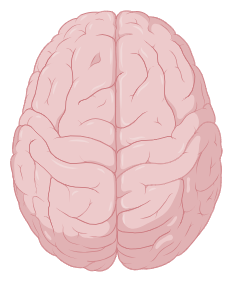
\includegraphics[scale=0.7]{Graphics/brain_pink}
     		\end{figure}
     		\end{column}
     		
     		\begin{column}{0.3\textwidth} % Left column width
     			\centering
     			Se encarga de recibir, interpretar y responder \\
     			a los est\'imulos del entorno.     			
     			
     		\end{column}
     	\end{columns} 	
        	
     	
     \end{frame}
 
   %------------------------------------------------
 	\begin{frame}
 		\frametitle{Especializaci\'on hemisf\'erica en la percepci\'on visual}
 		
 		\begin{columns}[c] % The "c" option specifies centered vertical alignment while the "t" option is used for top vertical alignment
 			\begin{column}{0.3\textwidth} % Right column width
 				\centering
 			\textbf{Hemisferio Izquierdo}\\ 					
 				
 			\end{column}
 			
 			\begin{column}{0.3\textwidth}
 				\centering
 				\begin{figure}     				
 					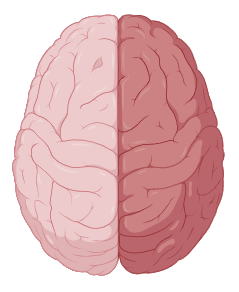
\includegraphics[scale=0.7]{Graphics/brain}
 				\end{figure}
 			\end{column}
 			
 			\begin{column}{0.3\textwidth} % Left column width
 				\centering
 				\textbf{Hemisferio Derecho}\\
 				
 			
 				
 				
 			\end{column}
 		\end{columns}
 		
 		
 	\end{frame}
 
	 %---------------------------------------------------------
 	
 	\begin{frame}
 		\frametitle{Niveles organizativos de las im\'agenes visuales} 		
 	
 	
 	\begin{columns}[c] % The "c" option specifies centered vertical alignment while the "t" option is used for top vertical alignment
 		\begin{column}{0.5\textwidth} % Right column width
 			\begin{figure}
 				\centering
 				
\includegraphics[scale=0.3]{Graphics/tree}
 			\end{figure}
 			\centering
 			\textbf{Global}\\
 			Percibir y procesar el conjunto o configuraci\'on general del est\'imulo visual.
 			
 			
 		\end{column}
 		
 		
 		\begin{column}{0.5\textwidth} % Left column width
 			\begin{figure}
 				\centering
 				
\includegraphics[scale=0.43]{Graphics/leaf_branch}
 			\end{figure}
 			\centering
 			\textbf{Local}\\
 			 Analizar y procesar los detalles específicos de un estímulo visual.		
 			
 		\end{column}
 	\end{columns}
 		
 		
 	\end{frame}
 
 	 %------------------------------------------------
 	\begin{frame}
 		\frametitle{Asimetr\'ia hemisf\'erica en la percepci\'on global/local}
 		
 		\begin{columns}[c] % The "c" option specifies centered vertical alignment while the "t" option is used for top vertical alignment
 			\begin{column}{0.3\textwidth} % Right column width
 				\centering
 			\textbf{Hemisferio Izquierdo}\\
 				$\downarrow$\\
 				\textbf{Percepci\'on Local}
 				
 				
 			\end{column}
 			
 			\begin{column}{0.3\textwidth}
 				\centering
 				\begin{figure}     				
 					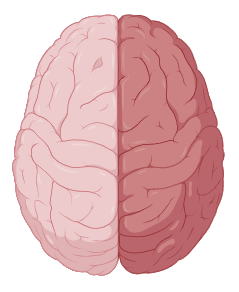
\includegraphics[scale=0.7]{Graphics/brain}
 				\end{figure}
 			\end{column}
 			
 			\begin{column}{0.3\textwidth} % Left column width
 				\centering
 				\textbf{Hemisferio Derecho}\\
 				
 				$\downarrow$\\
 				\textbf{Percepci\'on Global}
 				
 				
 			\end{column}
 		\end{columns}
 		
 		
 	\end{frame}
     
      %------------------------------------------------
    % \begin{frame}
    % 	\frametitle{Estudios sobre lateralizaci\'on hemisf\'erica}
    % 	
    % 	\begin{figure}
    % 		\centering
    % 		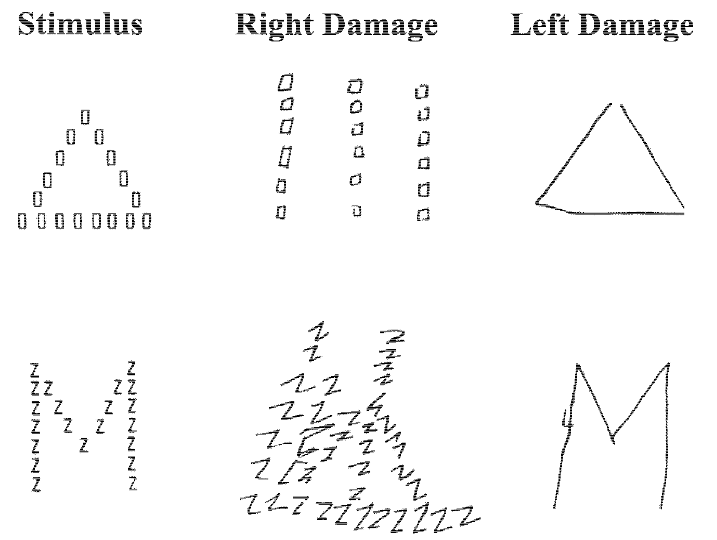
\includegraphics[scale=0.4]{Graphics/global_local}
    % 	\end{figure}
    %
    % 	
    % \end{frame}
     
    
     
     %------------------------------------------------
     \begin{frame}
     	\frametitle{Descomposici\'on de im\'agenes en componentes con diferentes frecuencias espaciales}   
     	
     	   	
     	\begin{columns}[c] % The "c" option specifies centered vertical alignment while the "t" option is used for top vertical alignment
     	\begin{column}{0.3\textwidth} % Right column width
     		\centering
     		\begin{figure}     				
     			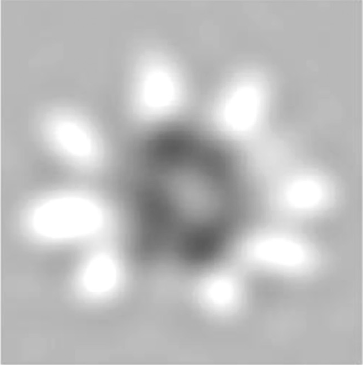
\includegraphics[scale=0.45]{Graphics/low_sf}
     		\end{figure}
     		\textit{Solo Frecuencias Bajas}
     		
     	\end{column}
     	
     	\begin{column}{0.3\textwidth}
     		\centering
     		\begin{figure}     				
     			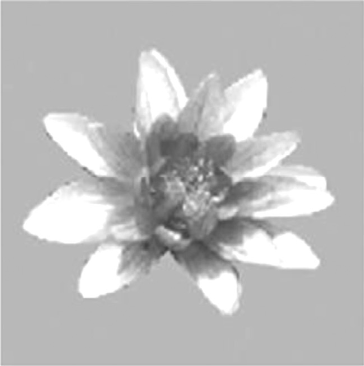
\includegraphics[scale=0.45]{Graphics/flower}
     		\end{figure}
     		\textit{Original}
     	\end{column}
     	
     	\begin{column}{0.3\textwidth} % Left column width
     		\centering
     		\begin{figure}     				
     			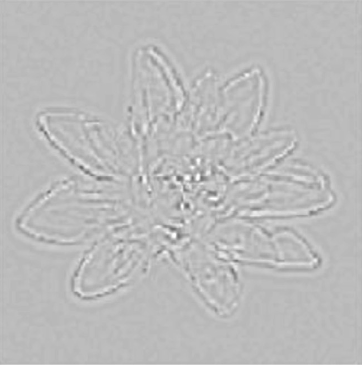
\includegraphics[scale=0.45]{Graphics/high_sf}
     		\end{figure}
     	
     	\textit{Solo Frecuencias Altas}    		
     		
     	\end{column}
     \end{columns}
    	
     	
     	
     \end{frame}
	
	%------------------------------------------------
	\begin{frame}
		\frametitle{Teor\'ia del Doble Filtraje por Frecuencia}
		
		\begin{columns}[t] % The "c" option specifies centered vertical alignment while the "t" option is used for top vertical alignment	
		
			\begin{column}{0.3\textwidth} % Left column width		
			\begin{figure}
				\captionsetup{font=tiny}
				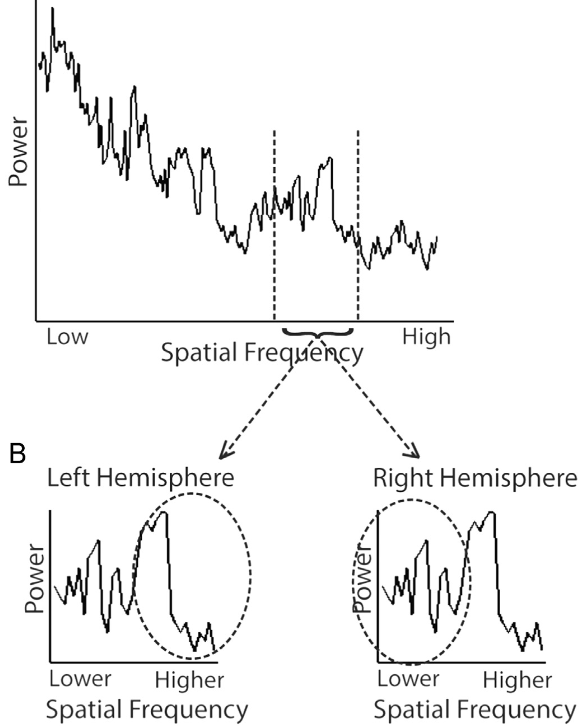
\includegraphics[scale=0.25]{Graphics/dff}
				\caption{Tomado de \cite{flevaris_spatial_2016}}
			\end{figure} 	
				
				
			\end{column}
		
		\begin{column}{0.4\textwidth} % Right column width
			\begin{enumerate}
				\item Seleccionar un rango de operación.
				\item Distribuir la información a los dos hemiferios.
			\end{enumerate}	
			
		\end{column}
		\end{columns}	
		
		
	\end{frame}
	%------------------------------------------------
	\begin{frame}
		\frametitle{Lateralizaci\'on hemisf\'erica respecto a frecuencias espaciales de est\'imulos visuales}
		
		\begin{columns}[c] % The "c" option specifies centered vertical alignment while the "t" option is used for top vertical alignment
			\begin{column}{0.3\textwidth} % Right column width
				\centering
				\textbf{Hemisferio Izquierdo}\\
				$\downarrow$\\
				\textbf{Percepci\'on Local}\\
				$\downarrow$\\
				\textbf{Frecuencias Espaciales Altas}
				
				
			\end{column}
			
			\begin{column}{0.3\textwidth}
				\begin{figure}
					\centering
					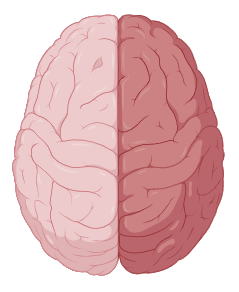
\includegraphics[scale=0.7]{Graphics/brain}
				\end{figure}
			\end{column}
			
			\begin{column}{0.3\textwidth} % Left column width
			\centering
			\textbf{Hemisferio Derecho}\\
			
			$\downarrow$\\
			\textbf{Percepci\'on Global}\\
				$\downarrow$\\
				\textbf{Frecuencias Espaciales Bajas}
				
				
			\end{column}
		\end{columns}
		
	
		
		
	\end{frame}


 %-----------------------------------------------------
	\begin{frame}
		\frametitle{}
		\textbf{A pesar de lo atractivo de la teor\'ia anterior, no se han identificado los mecanismos neurales que expliquen esta lateralizaci\'on hemisf\'erica del cerebro en la percepci\'on visual.}
		\newline
		
		

		
	\end{frame}

%-------------------------------------------
%-----------------------------------------------------
\begin{frame}
	\frametitle{}
	\textbf{A pesar de lo atractivo de la teor\'ia anterior, no se han identificado los mecanismos neurales que expliquen esta lateralizaci\'on hemisf\'erica del cerebro en la percepci\'on visual.}
	\newline
	
	La soluci\'on posiblemente este en la modelaci\'on de \textbf{campos receptivos poblacionales} y \textbf{mapas retinot\'opicos}.
	
	
	
\end{frame}

%-------------------------------------------
\begin{frame}
	\frametitle{Existen m\'as de 12 \'areas visuales con mapas retinot\'opicos}
	\begin{columns}[c] % The "c" option specifies centered vertical alignment while the "t" option is used for top vertical alignment
	\begin{column}{0.7\textwidth} % Right column width
	\begin{figure}
			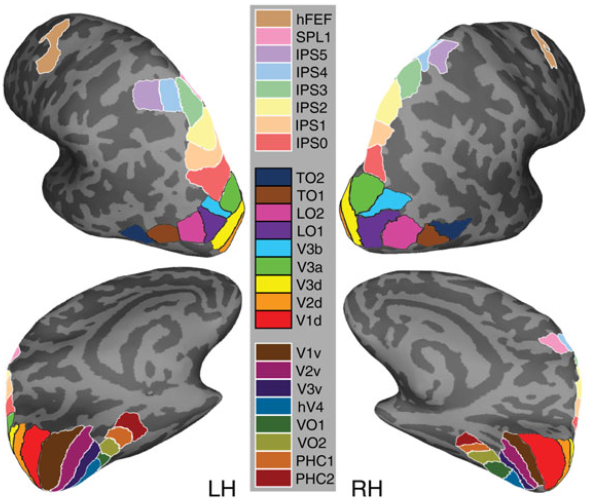
\includegraphics[scale=0.55]{Graphics/brain_wang}
		\captionsetup{font=tiny}
		\caption{Tomado de \cite{wang_probabilistic_2015}}
	\end{figure}	
		
	\end{column}
	
	\begin{column}{0.3\textwidth}
		
	\end{column}
	
	
\end{columns}
	
	

\end{frame}

%-------------------------------------------
\begin{frame}
	\frametitle{Existen m\'as de 12 \'areas visuales con mapas retinot\'opicos}
	\begin{columns}[c] % The "c" option specifies centered vertical alignment while the "t" option is used for top vertical alignment
		\begin{column}{0.7\textwidth} % Right column width
			\begin{figure}
				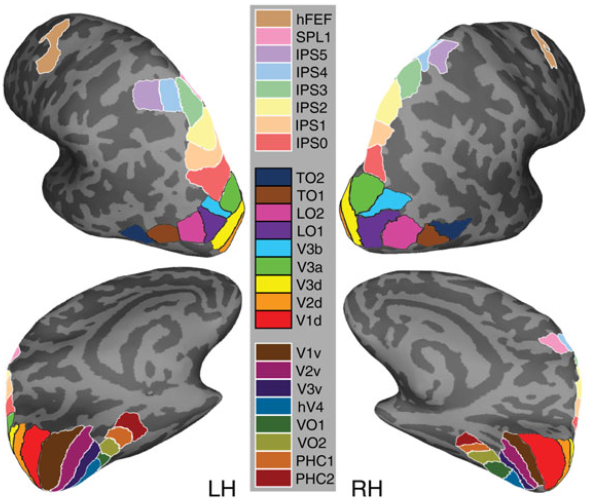
\includegraphics[scale=0.55]{Graphics/brain_wang}
				\captionsetup{font=tiny}
				\caption{Tomado de \cite{wang_probabilistic_2015}}
			\end{figure}	
			
		\end{column}
		
		\begin{column}{0.35\textwidth}
			\centering
		\textbf{\textit{¿En cu\'ales de estas \'areas se presenta lateralizaci\'on hemisf\'erica?}}
		\end{column}
		
		
	\end{columns}
	
	
	
\end{frame}
		
	%-------------------------------------------
	
	
\begin{frame}
	\frametitle{Campos Receptivos de Poblaciones Neurales}
	
	\begin{block}{}
		Modelos matemáticos que cuantifican y describen cómo las neuronas en un v\'ertice cortical responden a estímulos visuales. Estiman la \textbf{posición} y el \textbf{tamaño} del campo visual que afecta a un v\'ertice cortical.
	\end{block}
	
	\begin{columns}
		
		\begin{column}{0.5\textwidth}
			\begin{figure}
			\centering
			\captionsetup{font=tiny}
			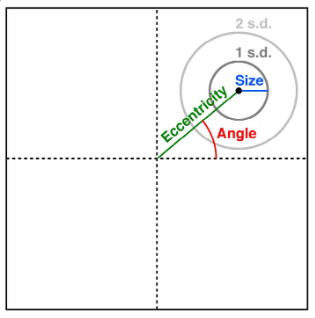
\includegraphics[scale=0.45]{Graphics/pRF2}
			\caption{Tomado de \cite{benson_human_2018}}
			\end{figure}
		\end{column}
		
		\begin{column}{0.5\textwidth} % Right column width
		
			
		\end{column}					
		
	\end{columns}
	
	
	
\end{frame}


%------------------------------------------------
\begin{frame}
	\frametitle{Campos Receptivos de Poblaciones Neurales}
	
	\begin{block}{}
		Modelos matemáticos que cuantifican y describen cómo las neuronas en un v\'ertice cortical responden a estímulos visuales. Estiman la \textbf{posición} y el \textbf{tamaño} del campo visual que afecta a un v\'ertice cortical.
	\end{block}
	
	\begin{columns}
		
		\begin{column}{0.5\textwidth}
			\begin{figure}
				\centering
				\captionsetup{font=tiny}
				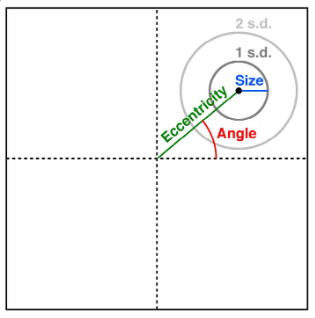
\includegraphics[scale=0.45]{Graphics/pRF2}
				\caption{Tomado de \cite{benson_human_2018}}
			\end{figure}
		\end{column}
		
		\begin{column}{0.5\textwidth} % Right column width
				\centering
			\textbf{\textit{¿En qu\'e difieren las propiedades de los campos receptivos en ambos hemisferios?}}
			
		\end{column}					
		
	\end{columns}
	
	
	
\end{frame}



%----------------------------------------------------------------
\begin{frame}
	\frametitle{Mapa Retinot\'opico Bayesiano}
	
	\begin{columns}
		
		\begin{column}{0.3\textwidth}
			El \textbf{mapa bayesiano} combina:
			\begin{itemize}
				\item Mediciones promedio de la población.
				\item Mediciones específicas de un sujeto.
			\end{itemize}	
		\end{column}
		
		\begin{column}{0.7\textwidth} % Right column width
		
			\begin{figure}
				
				\captionsetup{font=tiny}
				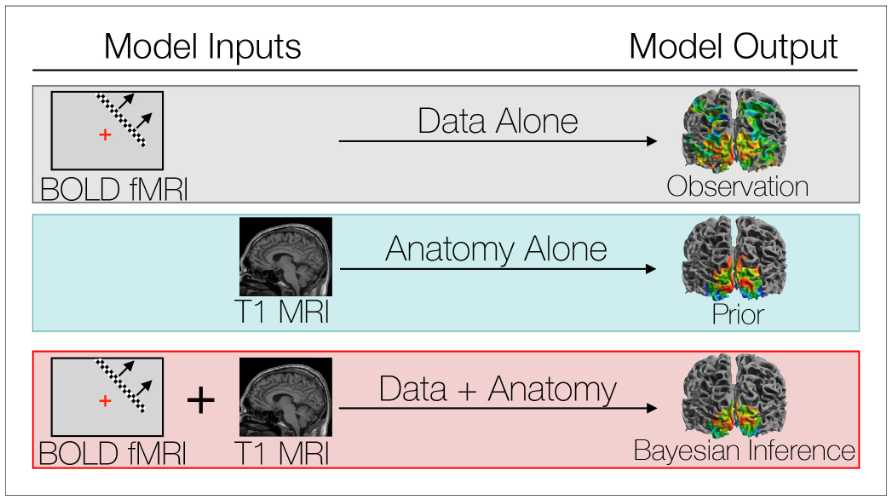
\includegraphics[scale=0.4]{Graphics/bayesian}
				\caption{Tomado de \cite{benson_bayesian_2018}}
			\end{figure}
		\end{column}					
		
	\end{columns}
	

	
\end{frame}
%-------------------------------------------------


	\section{Objetivos} % Sections are added in order to Organize your presentation into discrete blocks, all sections and subsections are automatically output to the table of contents as an overview of the talk but NOT output in the presentation as separate slides
	
	%------------------------------------------------
	\begin{frame}
		\frametitle{Objetivo General}
	\begin{columns}
		
		\begin{column}{0.2\textwidth}
			
		\end{column}
		
		\begin{column}{0.6\textwidth} % Right column width
			\centering
			\textbf{El objetivo general de este estudio es analizar la especializaci\'on hemisférica del cerebro para frecuencias espaciales mediante campos receptivos poblacionales.}
			
		\end{column}
		\begin{column}{0.2\textwidth} % Right column width
		
		
	\end{column}					
		
	\end{columns}
	
		
		
		%		
	\end{frame}
	
	\begin{frame}
		\frametitle{Objetivos Espec\'ificos}
		\begin{itemize}
			\item[1.]  Aplicar modelos que estiman la frecuencia espacial preferida de los v\'ertices corticales.
			
			\item[2.] Implementar modelos estadísticos para explicar las diferencias en las frecuencias preferidas de los v\'ertices corticales entre hemisferios.	
			
			\item[3.] Analizar la lateralización hemisférica en diferentes áreas visuales.
		\end{itemize}
		
		
		%		
	\end{frame}
	
	%------------------------------------------------
	\section{Materiales y M\'etodos}
	\begin{frame}
		\frametitle{Datos}
		
		
		Se utilizaron datos de 12 sujetos medidos por \cite{broderick_mapping_2022} estimulados con rejillas con diferente frecuencias espaciales.
			
		
	
		\begin{figure}
			\centering
			\captionsetup{font=tiny}
			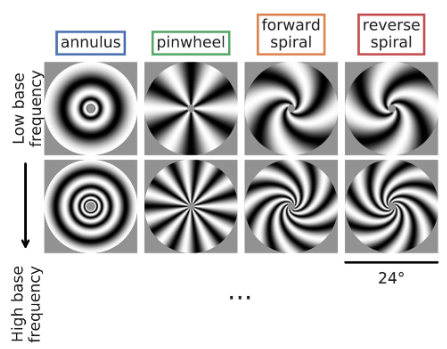
\includegraphics[scale=0.65]{Graphics/stimulus}
			\caption{Tomado de \cite{broderick_mapping_2022}}
		\end{figure}
		
		
		
	\end{frame}
	
	
	%------------------------------------------------
	\begin{frame}
		\frametitle{Tipos de Datos}
		
		Utilizando Resonancicia Magn\'etica Funcional se obtuvieron:
		\begin{itemize}
			\item Estimaciones de amplitud de respuesta de las activaciones neuronales, a los est\'imulos visuales.
			\item Soluciones de los \textit{Campos Receptivos de Poblaciones Neurales} (pRFs).
			\item \textit{Mapas Retinot\'opicos Bayesianos}.
			
		\end{itemize}	
		
	\end{frame}

	

	%------------------------------------------------
	\begin{frame}
		\frametitle{Estimaci\'on de per\'iodo preferido de \cite{broderick_mapping_2022}}
		
		
				\centering
				\begin{equation*}
					\hat{\beta}_b(w_l) = A_b \cdot \exp\left(\frac{-(\log_2(w_l) + \log_2(p_b))^2}{2\sigma_b^2}\right)					
				\end{equation*}	
				
				
		
				\begin{itemize} 			
					\item \(\hat{\beta}_b(w_l)\): Respuesta neurales promedio en el intervalo de excentricidad \(b\) a la frecuencia espacial \(w_l\).		
					\item \(A_b\): Ganancia de respuesta.
					\item \(p_b\): Per\'iodo preferido.
					\item \(\sigma_b\): Ancho de banda medido en octavas.
				\end{itemize}					
		
				
	\end{frame}
	
	%------------------------------------------------
	\section{Resultados}
	
	\begin{frame}
		\frametitle{}
		\centering
	 	\textbf{ \Huge{Resultados}}
	\end{frame}
	%------------------------------------------------
	\begin{frame}
		\frametitle{Tama\~no de pRF crece con la excentricidad}
		
		\begin{columns}[t] % The "c" option specifies centered vertical alignment while the "t" option is used for top vertical alignment
			
			
			\begin{column}{0.7\textwidth}
				\begin{figure}
					\centering
				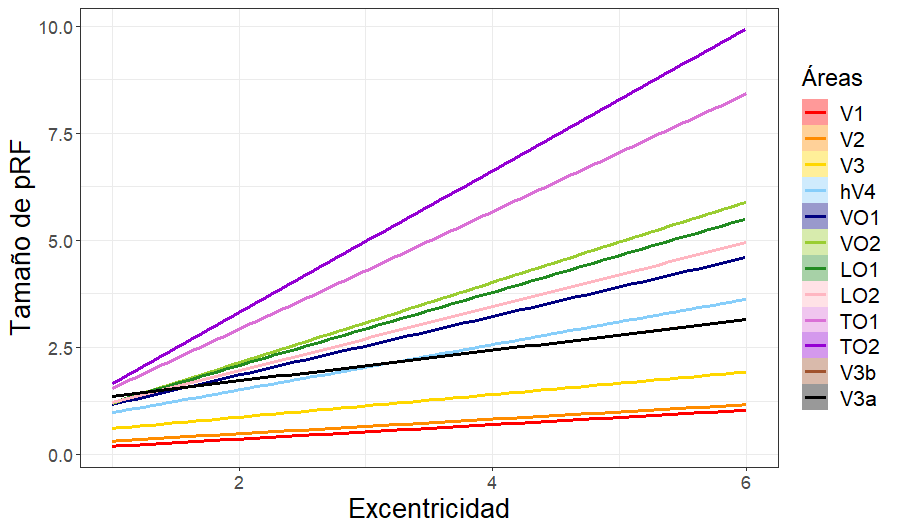
\includegraphics[scale=0.5]{../../../thesis_temp/document/Graphics/size_vs_eccen_bayesian}
				\end{figure}
			\end{column}
		
			\begin{column}{0.3\textwidth} % Right column width
				\begin{itemize}
					\item El tama\~no de los pRFs crece con la excentricidad.
					\item La pendiente es mayor en \'areas visuales superiores (TO2).
					
				\end{itemize}
				
				
				
			\end{column}					
			
		\end{columns}
		
	\end{frame}
	
	%------------------------------------------------
	\begin{frame}
		\frametitle{Per\'iodo preferido y excentricidad}
		
			\begin{columns}[t] % The "c" option specifies centered vertical alignment while the "t" option is used for top vertical alignment
			
			
			\begin{column}{0.7\textwidth}
				\begin{figure}
					
					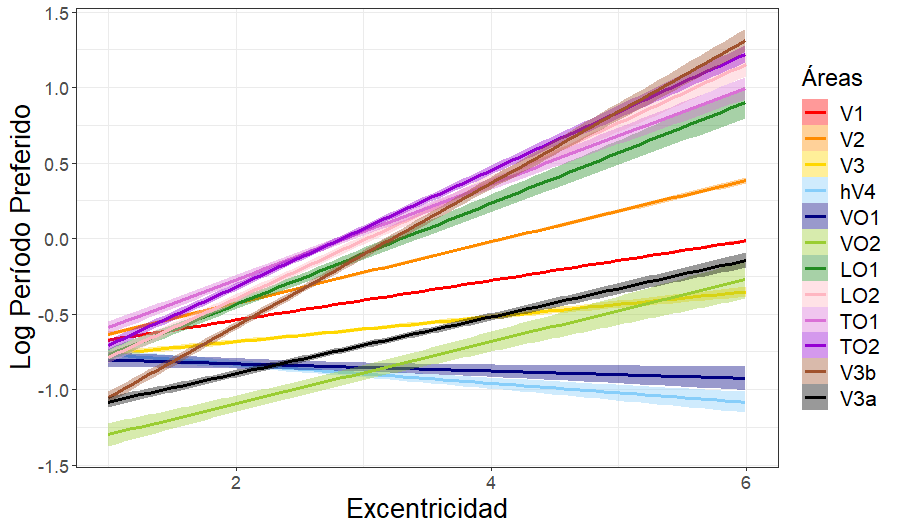
\includegraphics[scale=0.5]{../../../thesis_temp/document/Graphics/pp_vs_eccen}
				\end{figure}
			\end{column}
			
			\begin{column}{0.3\textwidth} % Right column width
				\begin{itemize}
					\item Per\'iodo preferido crece en mayor\'ia de \'areas.
					\item Pendiente mayor en \'areas visuales superiores.
					
				\end{itemize}
				
				
				
			\end{column}					
			
		\end{columns}
				
		
		
	\end{frame}
	
	%------------------------------------------------
	%------------------------------------------------
	\begin{frame}
		\frametitle{Modelo lineal mixto para per\'iodo preferido de v\'ertices corticales}
		
		Se construy\'o un modelo lineal mixto que explica las relaciones anteriores, as\'i como la lateralizaci\'on hemisf\'erica del cerebro.
		
		\begin{equation*}
			\text{Período Preferido} \sim  \text{Excentricidad} \times \text{Hemisferio} + (1 | \text{Sujeto}) + (1 | \text{Estímulo})	
			\label{mlm_pp}
		\end{equation*}
		
	\end{frame}

	\begin{frame}
		\frametitle{Tama\~no de efecto de variables fijas del modelo}	
		
			
			 \begin{itemize}
			 	\item Efecto de la \textbf{excentricidad} notable en áreas superiores como TO1 y TO2.
			 	\item La interacción \textbf{excentricidad:hemisferio} es pequeña en todas  las áreas.
			 	\item Efecto del \textbf{hemisferio} es grande en hV4, VO1, LO1 y muy pequeño en LO2.
			 \end{itemize}
		
				\begin{figure}
					\centering
					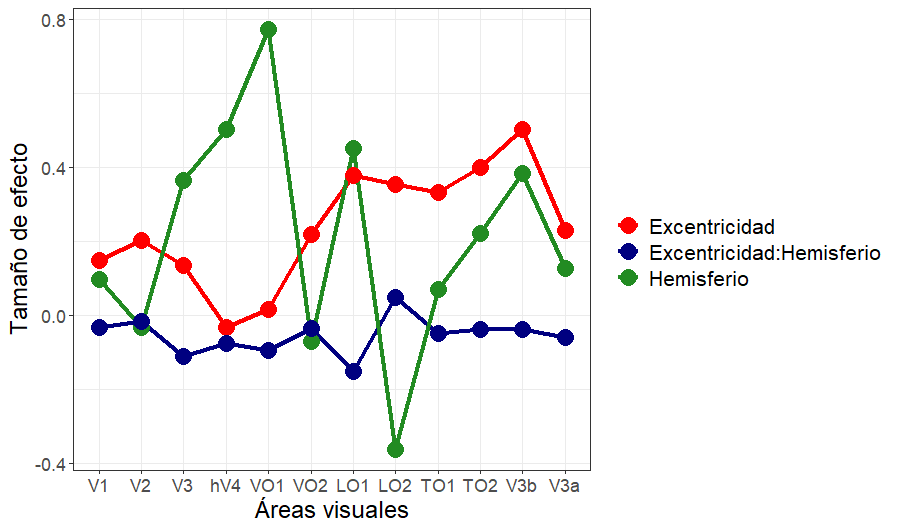
\includegraphics[scale=0.35]{Graphics/effect_size_coef_pp}
				\end{figure}				
				
		
		
	
		
		
	\end{frame}

	\begin{frame}
		\frametitle{Resultados del modelo respecto a los hemisferios}
		
		La diferencia entre hemisferios es m\'as pronunciada en las áreas hV4 y VO1.		
			
			\begin{figure}
				\centering
			 	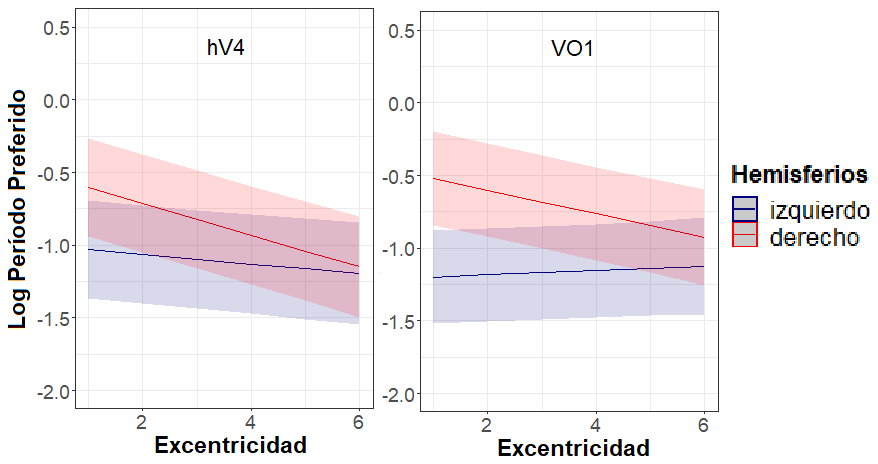
\includegraphics[scale=0.5]{Graphics/hv4}
			\end{figure}
	
	\end{frame}

	
	%------------------------------------------------
	%\section{Modelos}
	
	%------------------------------------------------
	
	%------------------------------------------------
	%\begin{frame}
	%	\frametitle{Modelo lineal mixto}	
	%	
	%	
	%	\begin{itemize}
	%		\item \textbf{Modelo Nulo:}	\\			
	%		\begin{equation*}
	%			\text{Período Preferido} \sim 1 + (1 | \text{Sujeto}) + (1 | \text{Estímulo})	
	%			\label{m_1}
	%		\end{equation*}
	%		
	%		\item\textbf{Modelo con Excentricidad:}\\			
	%		\begin{equation*}
	%			\text{Período Preferido} \sim \text{Excentricidad} + (1 | \text{Sujeto}) + (1 | \text{Estímulo})	
	%			\label{m_2}
	%		\end{equation*}
	%		
	%		\item \textbf{Modelo Aditivo con Excentricidad y Hemisferio:}\\				
	%		\begin{equation*}
	%			\text{Período Preferido} \sim \text{Excentricidad} + \text{Hemisferio} + (1 | \text{Sujeto}) + (1 | \text{Estímulo})	
	%			\label{m_3}
	%		\end{equation*}
	%		
	%		\item \textbf{Modelo con Interacci\'on de Excentricidad y Hemisferio:}\\				
	%		
	%		
	%		
	%	\end{itemize}
	%	
	%	
	%\end{frame}
	
	%------------------------------------------------
		%------------------------------------------------

	
	%------------------------------------------------
	
	%------------------------------------------------
	%------------------------------------------------

	%------------------------------------------------
	\section{Conclusión}
	%------------------------------------------------
	
	\begin{frame}
		\frametitle{Conclusiones}
		
	
		
	\end{frame}

		\begin{frame}
		\frametitle{Conclusiones}
		
		\begin{minipage}[t][0.8\textheight][t]{\textwidth}
			\begin{itemize}
				\item[1.] Se estim\'o el período preferido (el inverso de la frecuencia espacial preferida) de los vértices corticales en diferentes áreas visuales.
				
			\end{itemize}
		\end{minipage}
		
		
		
	\end{frame}

		\begin{frame}
		\frametitle{Conclusiones}
			\begin{minipage}[t][0.8\textheight][t]{\textwidth}
			\begin{itemize}
				\item[1.] Se estim\'o el período preferido (el inverso de la frecuencia espacial preferida) de los vértices corticales en diferentes áreas visuales.
				\item  [2.] Se utiliz\'o un modelo lineal mixto para interpretar los resultados del período preferido estimado.
			\end{itemize}
		\end{minipage}
		
		
	\end{frame}

		\begin{frame}
		\frametitle{Conclusiones}
			\begin{minipage}[t][0.8\textheight][t]{\textwidth}
			\begin{itemize}
				 \item[1.] Se estim\'o el período preferido (el inverso de la frecuencia espacial preferida) de los vértices corticales en diferentes áreas visuales.
				\item  [2.] Se utiliz\'o un modelo lineal mixto para interpretar los resultados del período preferido estimado.
				\item [3.] Se observ\'o que el período preferido de los v\'ertices corticales varía entre los hemisferios cerebrales en diversas áreas visuales, lo cual est\'a en consonancia con datos neurofisiológicos y neuropsicológicos previos  sobre la lateralización hemisférica.
			\end{itemize}
		\end{minipage}
	
		
	\end{frame}

	\begin{frame}
		\frametitle{Recomendaciones}
		
	\end{frame}
       
    \begin{frame}
    	\frametitle{Recomendaciones}
    	\begin{minipage}[t][0.8\textheight][t]{\textwidth}
    		\begin{itemize}
    				\item [1.] Revisar los datos actuales utilizando diferentes atlas retinotópicos.
    			
    		\end{itemize}
    	\end{minipage}
    	
   \end{frame} 
    \begin{frame}
    	\frametitle{Recomendaciones}
    	
    	\begin{minipage}[t][0.8\textheight][t]{\textwidth}
    		\begin{itemize}
    			\item [1.] Revisar los datos actuales utilizando diferentes atlas retinotópicos.
    		
    		\item [2.] Desarrollar simulaciones con redes neuronales convolucionales que incorporen los parámetros fisiológicos de este estudio. 
    		
    			
    		\end{itemize}
    	\end{minipage}
    	
    	 
    \end{frame}
    \begin{frame}
    	\frametitle{Recomendaciones}
    	
    	\begin{minipage}[t][0.8\textheight][t]{\textwidth}
    		\begin{itemize}
    			\item [1.] Revisar los datos actuales utilizando diferentes atlas retinotópicos.
    		
    			\item [2.] Desarrollar simulaciones con redes neuronales convolucionales que incorporen los parámetros fisiológicos de este estudio. 
    		
    			\item[3.] Aplicar la metodología de investigación a un conjunto de datos más amplio para obtener resultados más sólidos y confiables.
    			
    		\end{itemize}
    	\end{minipage}
    	
   \end{frame} 
    \begin{frame}
    	\frametitle{Recomendaciones}
    	
    		\begin{minipage}[t][0.8\textheight][t]{\textwidth}
    		\begin{itemize}
    			\item [1.] Revisar los datos actuales utilizando diferentes atlas retinotópicos.
    		
    		\item [2.] Desarrollar simulaciones con redes neuronales convolucionales que incorporen los parámetros fisiológicos de este estudio. 
    		
    		\item[3.] Aplicar la metodología de investigación a un conjunto de datos más amplio para obtener resultados más sólidos y confiables.
    		
    		\item[4.] Realizar experimentos de fMRI enfocados en medir la preferencia por distintas frecuencias espaciales en ambos hemisferios teniendo en cuenta la variación en el espectro de los estímulos visuales con la atenci\'on. 
    			
    		\end{itemize}
    	\end{minipage}
    
    \end{frame}
   
	


	\begin{frame}
		\frametitle{Preguntas}
			
		
	\end{frame}

	\begin{frame}
	\frametitle{Preguntas}
	\begin{itemize}
		\item[1.] Valore como pudiera afectar los resultados obtenidos en este estudio la elección de otro tipo de atlas cerebral. ¿Es posible que la delimitación de las áreas juegue un papel en el subconjunto de resultados negativos del estudio?	
		
		
	\end{itemize}     
	
	
	
	
\end{frame}

\begin{frame}
	\frametitle{Atlas Cerebral}
	
		\begin{columns}[t] % The "c" option specifies centered vertical alignment while the "t" option is used for top vertical alignment			
		\begin{column}{0.5\textwidth} % Left column width
			
			\begin{figure}			
				\centering
				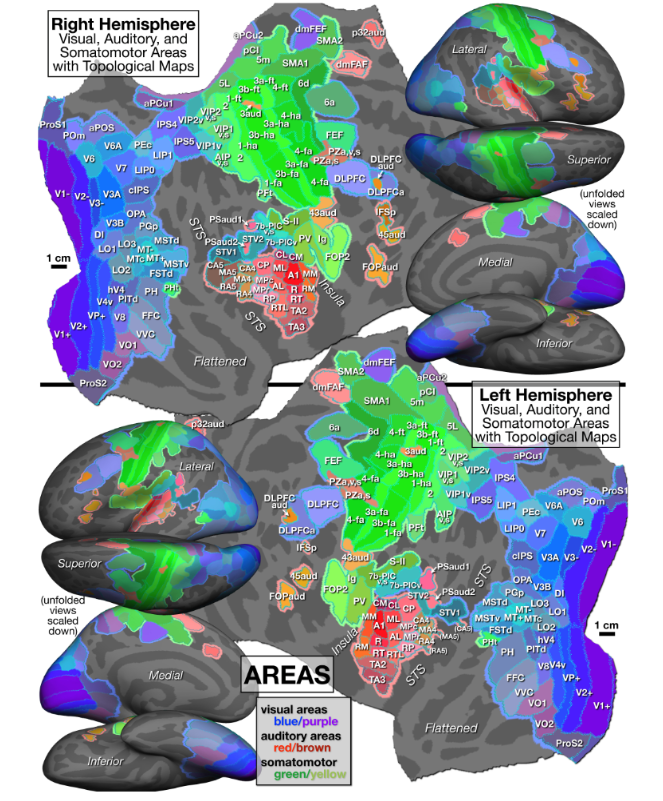
\includegraphics[scale=0.25]{Graphics/sereno}
				\captionsetup{font=tiny}
				\caption{Tomado de \cite{sereno_topological_2022}}
			\end{figure}		
		\end{column}
		\begin{column}{0.5\textwidth} % Right column width
		\begin{figure}			
			\centering
			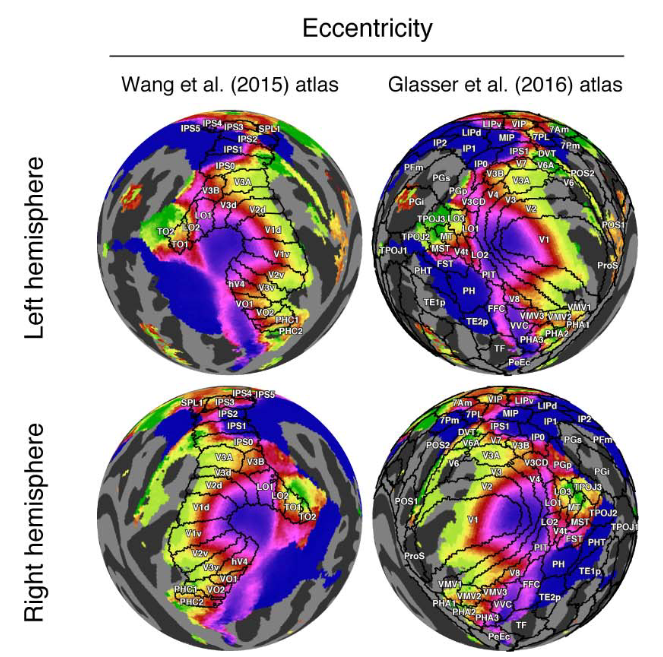
\includegraphics[scale=0.35]{Graphics/glasser_wang_eccen}
			\captionsetup{font=tiny}
			\caption{Tomado de \cite{benson_human_2018}}
		\end{figure}
			
			
		\end{column}
		
	
		
		
	\end{columns}
	


\end{frame}

	\begin{frame}
	\frametitle{Preguntas}
	\begin{itemize}		
		
		\item[2.] Resulta curioso que el efecto de disminución del logaritmo del período preferido con respecto a la excentricidad en hV4 y VO1 parece estar concentrado en el hemisferio derecho. ¿Pudiera comentar este resultado?	 
		
	\end{itemize}     
	
	
	
	
\end{frame}

\begin{frame}
	\frametitle{Resultado hemisferios en hV4 y VO1}
	
		\begin{figure}			
		\centering
		\includegraphics[scale=0.5]{Graphics/hV4}
		\captionsetup{font=tiny}
		
	\end{figure}
	
\end{frame}

\begin{frame}
	\frametitle{Resultado hemisferios en hV4 y VO1}
	

		\begin{figure}			
			\centering
			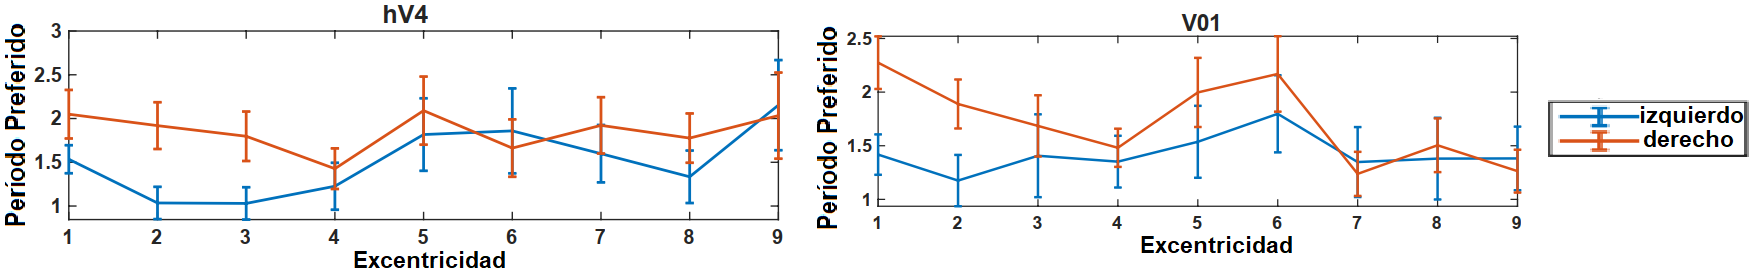
\includegraphics[scale=0.4]{Graphics/hv4_VO1}
						
		\end{figure}
		
	
	
\end{frame}



	
	\begin{frame}
	\frametitle{Referencias}
	     
	\bibliographystyle{apalike}
	\bibliography{biblio}
	
	
	
	\end{frame}
	
\end{document} 
